\section{Grafika komputerowa 3D}
% Fit the following in the main chapter
%\subsection{Procesory graficzne}
%\subsection{OpenGL}
%\subsection{Potok renderowania}
%\subsection{Shadery}
%\subsection{Cieniowanie}

Poniżej opisane zostaną podejścia wykorzystane do wyświetlenia trójwymiarowej symulacji opisanej poprzednim rozdziale.

\subsection{Renderowanie oparte na fizyce}

Renderowanie oparte na fizyce (ang. Physically Based Rendering, PBR) to podejście wykorzystywane w renderowaniu grafiki, które ma na celu wierne odwzorowanie zachowania światła oraz różnych materiałów.
\\

Przed wyłożeniem teorii warto się skupić, na jakim wejściu operować będzie nasz model. Z racji, że chcemy przybliżyć zachowanie światła zgodne z fizyką, to chcielibyśmy określać materiały za pomocą ich fizycznych właściwości. Zaimplementowany nami model oświetlenia obsługuje tekstury albedo, metaliczności, chropowatości, ambient occlusion oraz modyfikację wektorów normalnych.
Albedo, a więc kolor podstawowy, określa barwę, jaką światło będzie mieć po rozproszeniu na powierzchni materiału. Chropowatość mówi o tym, jak bardzo światło jest rozpraszane, a  metaliczność o tym, jaki udział mają efekty ciała dielektrycznego, a jakie przewodnika. Ambient occlusion oznacza poziom wystawienia powierzchni na oświetlenie otoczenia pozwalając na imitację gorzej doświetlonych szczelin. Wykorzystanie map normalnych pozwala natomiast na uzyskanie złudzenia większej złożoności modelu trójwymiarowego przy mniejszej liczbie wielokątów. Wektory normalne przed rozpoczęciem obliczeń dla każdego fragmentu są modyfikowane na podstawie tej mapy.
\\

Powyżej wymienione materiały są reprezentowane przez tekstury UV, gdzie każdy teksel koduje za pomocą trójki RGB wartość parametru dla konkretnego obszaru trójwymiarowego modelu. Na rysunku (\ref{pbrMaterial}) zaprezentowana jest przykładowa tekstura gdzie ambient occlusion jest zakodowane w kanale czerwonym, chropowatość w zielonym, a metaliczność w niebieskim. Obok, na rysunku (\ref{pbrNormal}) widnieje mapa normalnych w przestrzeni stycznej, na której trójki RGB zawierają informacje o odchyleniu względem wektora normalnego określonego przez geometrię modelu. 
\\


\begin{figure}[h]
	\centering
	\setkeys{Gin}{width=\textwidth}
	\begin{tabular}{p{0.45\textwidth}p{0.45\textwidth}}
		\copyrightbox[r]{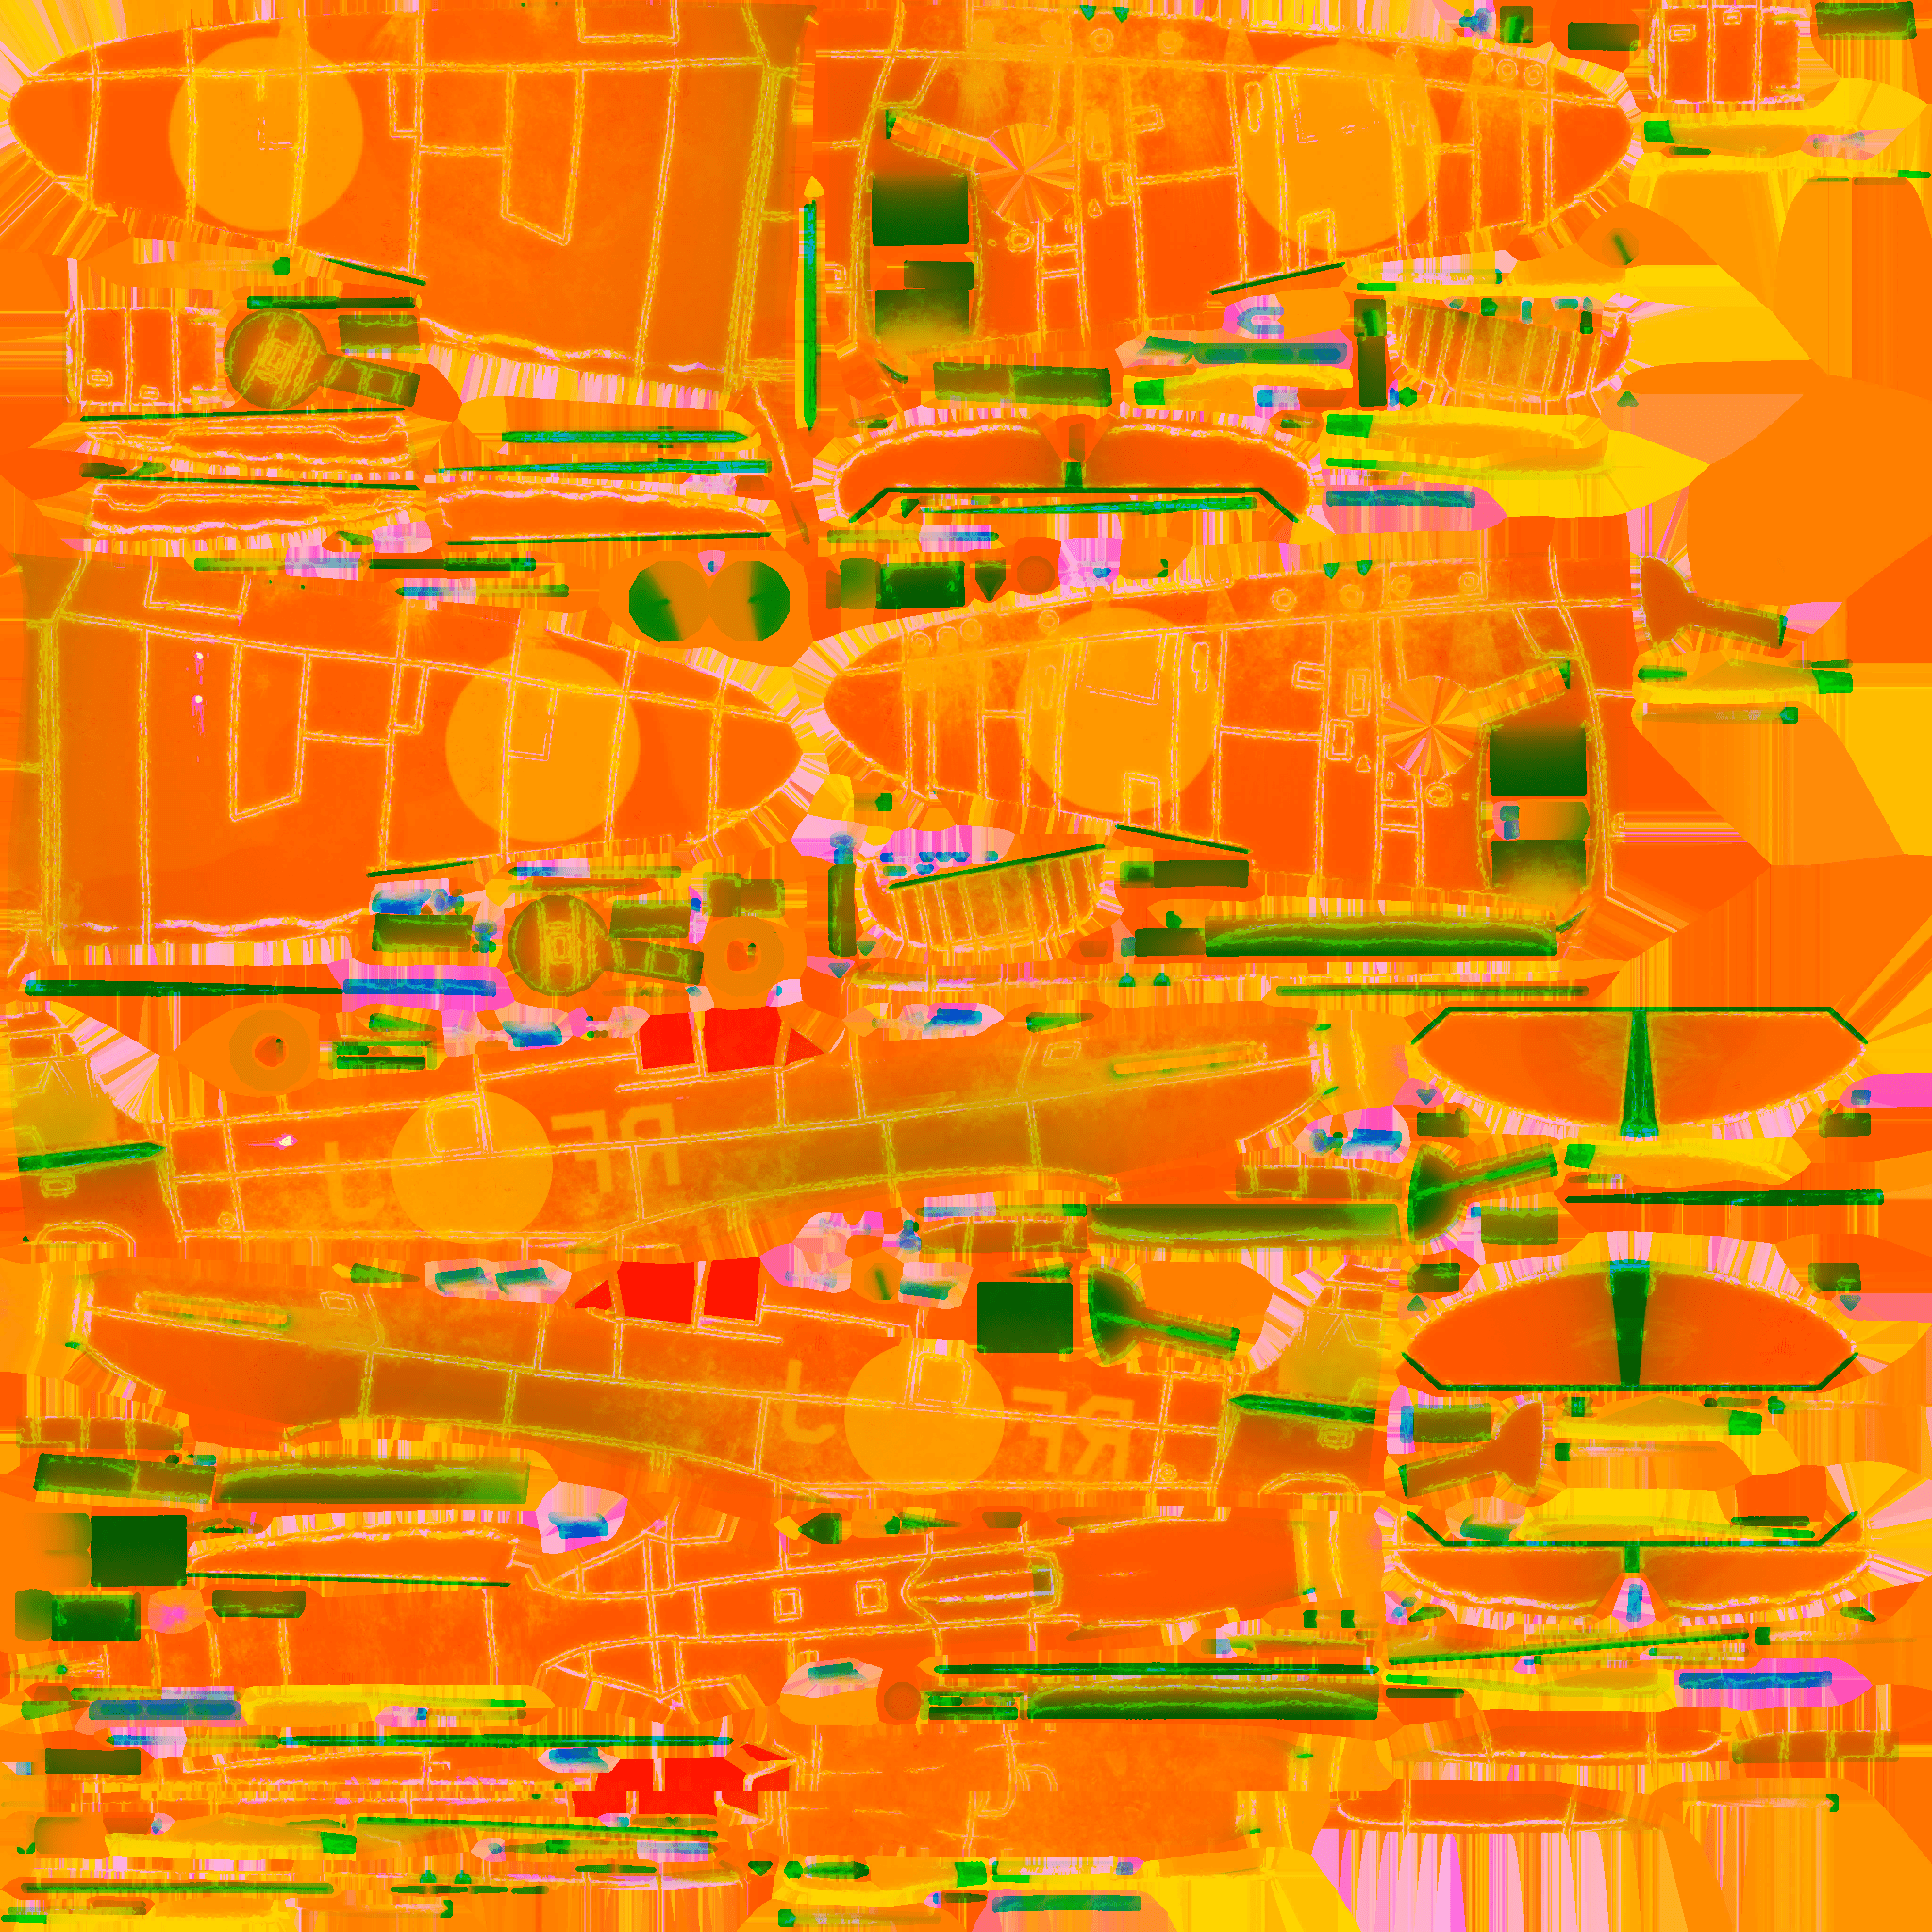
\includegraphics[width=0.4\textwidth]{pbrMaterial.png}}{\textcopyright kryik1023\\Sketchfab }
		& 
		\copyrightbox[r]{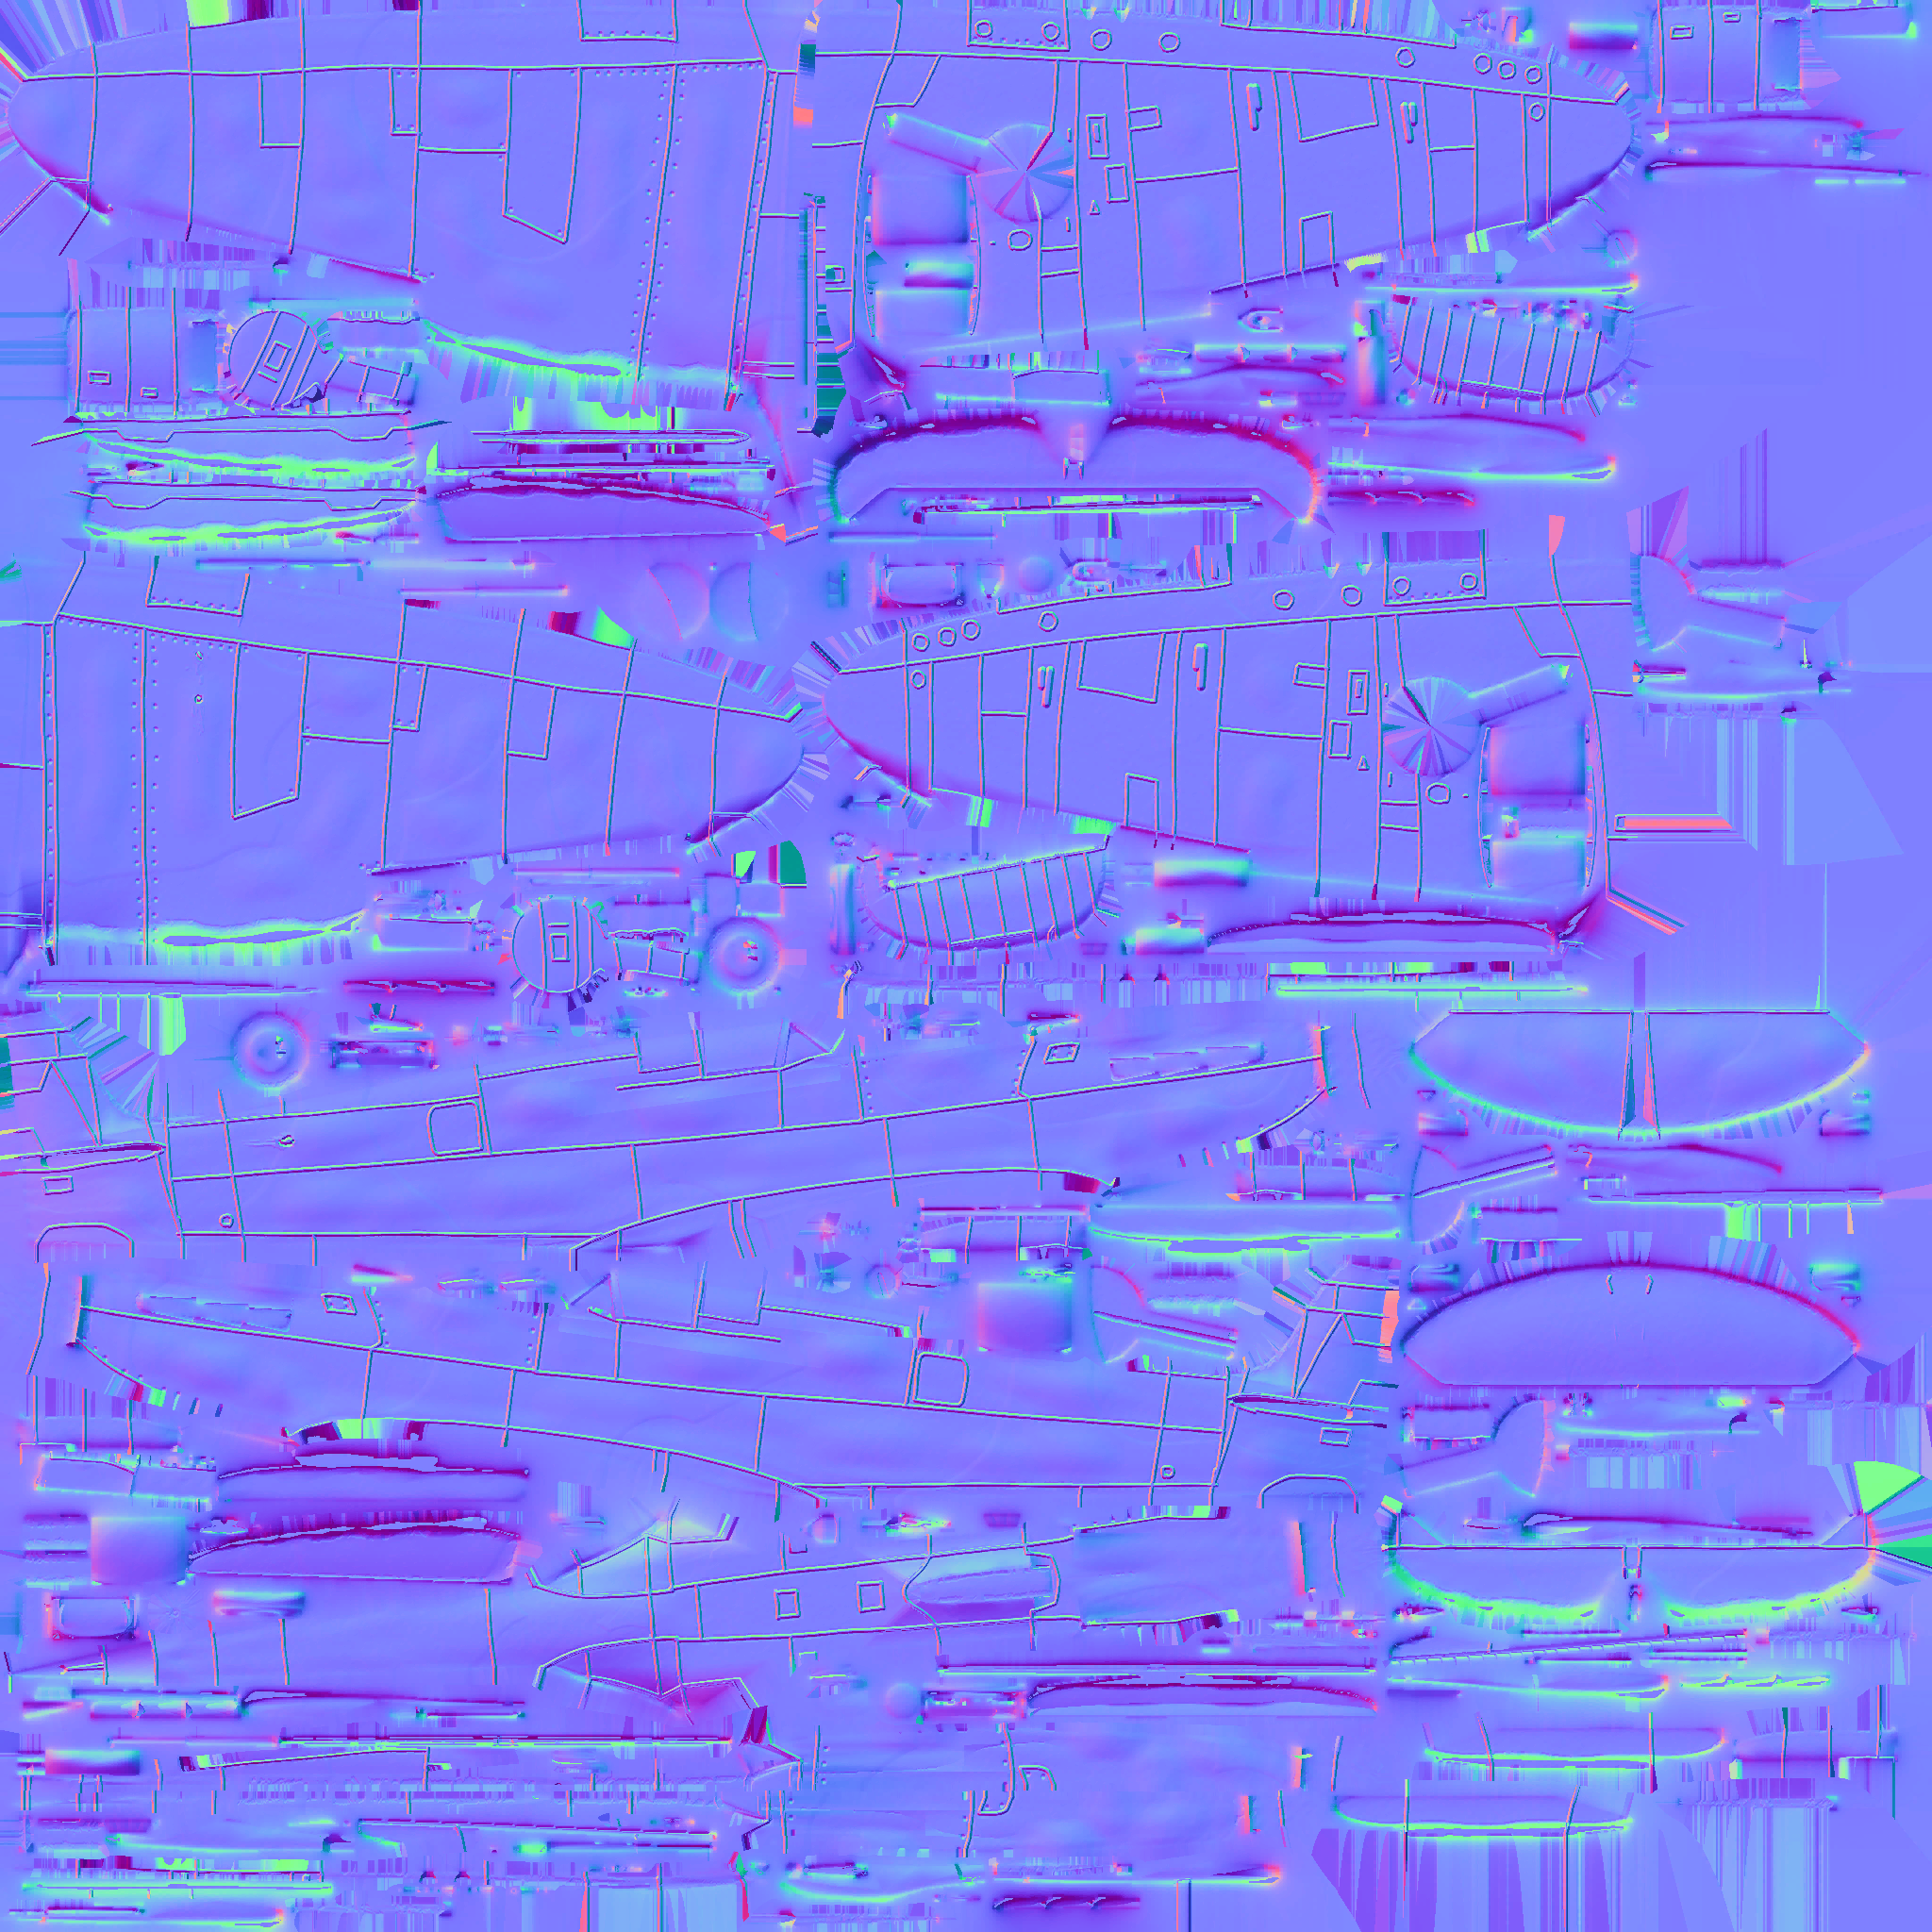
\includegraphics[width=0.4\textwidth]{pbrNormal.png}}{\textcopyright kryik1023\\Sketchfab }
		\\
		\caption{Przykładowy materiał wykorzystywany w PBR kodujący ambient occlusion w kanale czerwonym, chropowatość w zielonym, a metaliczność w niebieskim.}
		\label{pbrMaterial}
		&   \caption{Przykładowa mapa normalnych w przestrzeni stycznej.}
		\label{pbrNormal}
	\end{tabular}
\end{figure}

Jednym z problemów podejścia PBR jest wymóg zapewnienia dodatkowych tekstur określających parametry fizyczne. Ich brak może doprowadzić do dysonansu między modelami bardziej i mniej dopracowanymi.
\\

W przypadku naszej implementacji napisanej na podstawie \cite{learnopengl} założono, że będzie ono opierało się na modelu mikropowierzchni, zasady zachowania energii, wykorzystywało funkcję BRDF bazującą na fizyce oraz tym, co będzie to wszystko spajało, a więc równanie renderowania (ang. rendering equation). 
\\

Model mikropowierzchni został po raz pierwszy zaproponowany przez Roberta Cooka i Kennetha Torrance'a w 1982 roku \cite{cookTorrance}. Zakłada on, że każda powierzchnia w mikroskopijnej skali może zostać opisana poprzez zestaw małych doskonałych zwierciadeł ustawionych pod różnymi kątami nazywanych mikropowierzchniami. Wtedy, gładkość powierzchni materiału może zostać opisana poprzez proporcję mikropowierzchni, które w przybliżeniu są ustawione zgodnie z pewnym wektorem $h$. Tym wektorem jest wektor połowicznej drogi (ang. halfway vector) między wektorem światła $l$ oraz wektorem obserwatora $v$, który wyznacza się zgodnie z równaniem:

$$
	h= \frac{l + v}{\|l + v\|}.
$$

	
Mając powyższy model na uwadze możemy zaimplementować bazującą na nim funkcję BRDF (ang. Bidirectional Reflectance Distribution Function, dwukierunkową funkcję rozkładu odbicia). Charakteryzuje ona własności refleksyjne powierzchni odbijającej i pozwala na wyznaczenie stosunku radiancji, która trafi do obserwatora z badanego źródła światła po odbiciu od rozważanego punktu na powierzchni. Została ona po raz pierwszy zdefiniowana przez Freda Nicodemusa w 1965 \cite{Nicodemus} w następujący sposób:

$$
	f_r(\omega_i, \omega_o) = \frac{dL_o(\omega_o)}{dE_i(\omega_i)} = \frac{dL_o(\omega_o)}{L_i(\omega_i) cos(\theta_i) d(\omega_i)},
$$

gdzie $L_i(\omega_i)$ oraz $E_i(\omega_i)$ oznaczają radiancję i irradiancję w kierunku światła $\omega_i$, $L_o(\omega_o)$ radiancję w kierunku obserwatora $\omega_o$, a $\theta_i$ oznacza kąt między kierunkiem światła $\omega_i$ oraz wektorem normalnym powierzchni odbijającej $n$. 
\\ 

Implementacja funkcji zaproponowana przez Cooka i Torrace'a ma następującą postać:

$$
f_r(\omega_i, \omega_o) = k_d \frac{c}{\pi} + k_s\frac{D \cdot F \cdot G}{4\left(\omega_o \cdot n \right) \left( \omega_i \cdot n \right)}
$$

Suma składa się z dwóch składowych: składowej rozproszonej i zwierciadlanej. $\frac{c}{\pi}$ odpowiada znormalizowanemu odbiciu lambertowskiemu, gdzie $c$ oznacza albedo, a więc zdolność odbijania światła przez daną powierzchnię. Jest to kolor, jaki miałaby idealnie matowa powierzchnia. Składowa zwierciadlana bierze pod uwagę trzy czynniki, które normalizuje w mianowniku. Są nimi:
\begin{enumerate}
	\item $D$ -- Funkcja rozkładu wektorów normalnych aproksymująca liczbę mikropowierzchni, które są zgodne z wektorem $h$,
	\item $G$ -- Funkcja geometrii opisująca jak bardzo mikropowierzchnie zasłaniają siebie nawzajem, blokując światło przychodzące i wychodzące,
	\item $F$ -- Równanie Fresnela opisujące odbicie światła, gdy pada ono na granicę między różnymi ośrodkami optycznymi.
\end{enumerate}

Wykorzystaną funkcją rozkładu wektorów normalnych jest Trowbridge-Reitz GGX, która wygląda następująco:

$$
NDF_{GGXTR}(n,h,\alpha) = \frac{\alpha^2}{\pi\left( (n\cdot h)^2 (\alpha^2 - 1) + 1 \right)^2 },
$$
gdzie $\alpha$ oznacza miarę chropowatości powierzchni. Na rysunku (\ref{normaldistribution}) pokazany został efekt funkcji w zależności od chropowatości.


\begin{figure}[h]
	\centering
	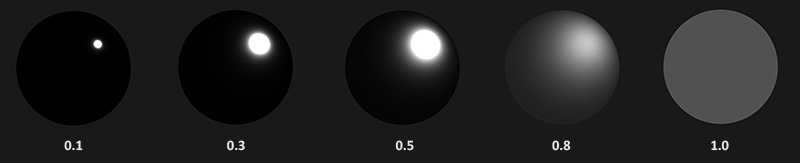
\includegraphics[width=1\textwidth]{ndf.png}
	\caption{Prezentacja funkcji rozkładu wektorów normalnych Trowbridge-Reitz GGX dla różnych wartości chropowatości. Widać, że im mniejsza chropowatość tym więcej mikropowierzchni zgodnych z wektorem $h$ jest skoncentrowane na mniejszej powierzchni}
	\label{normaldistribution}
\end{figure}

Funkcja geometryczna, podobnie jak powyższa, przyjmuje parametr chropowatości. Zakłada ona, że im powierzchnia jest bardziej chropowata, tym częściej jedne mikropowierzchnie będą zasłaniać drugie, co można zaobserwować na rysunku (\ref{geometry_shadowing}). Zjawisko to będzie wyznaczane na podstawie poniższej funkcji znanej jako Schlick-GGX:

$$
G_{SchlickGGX}(n,v,\alpha) = \frac{n \cdot v}{(n\cdot v)(1-k) + k)}, \hspace{1em} k = \frac{(\alpha+1)^2}{8},
$$
Aby uwzględnić blokowanie światła przychodzącego i wychodzącego wykorzystamy metodę Smitha:

$$
G(n, l, v, \alpha)  = G_{SchlickGGX}(n,v,\alpha)G_{SchlickGGX}(n,l,\alpha),
$$
gdzie $v$ oznacza wektor w kierunku obserwatora. Efekt funkcji jest widoczny na rysunku (\ref{geometry}).

\begin{figure}[h]
	\centering
	
\includegraphics[width=0.5\textwidth]{geometry_shadowing.png}
	\caption{Przykład zasłaniania części światła przez chropowatość powierzchni \cite{learnopengl}.}
	\label{geometry_shadowing}
\end{figure}


\begin{figure}[h]
	\centering
	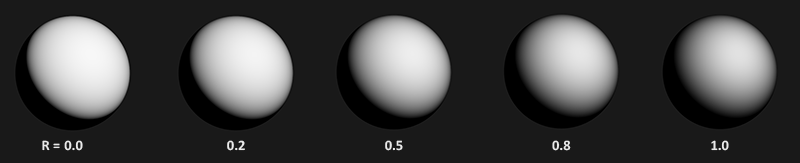
\includegraphics[width=1\textwidth]{geometry.png}
	\caption{Prezentacja funkcji geometrycznej Schlick-GGX w zależności od wartości chropowatości \cite{learnopengl}.}
	\label{geometry}
\end{figure}

Ostatnia z trzech funkcji, czerpiąca z równania Fresnela, które określają fenomen, w którym każda płaszczyzna wydaje się odbijać światło, jeżeli jest widziana pod dostatecznie dużym kątem. W naszej implementacji zostanie wykorzystana aproksymacja Schlick'a:

\[
	F_{Schlick}(h, v, F_0) = F_0 + (1-F_0)(1-(h\cdot v))^5.
\]

$F_0$ w powyższym równaniu oznacza podstawowy współczynnik odbicia, który aproksymuje się zazwyczaj jako trójkę $(0.04,0.04,0.04)$. Jeżeli dodatkowo materiał jest metalem, to interpolujemy tą wartość z kolorem bazowym materiału na podstawie parametru metaliczności. Tą metodą otrzymujemy dostatecznie realistyczne efekty bez dużego komplikowania ciężkimi obliczeniami. Na rysunku (\ref{fresnel}) można zaobserwować jak wygląda przykładowy efekt równania fresnela.
\\

\begin{figure}[h]
	\centering
	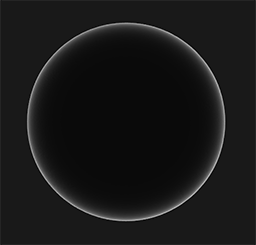
\includegraphics[width=0.3\textwidth]{fresnel.png}
	\caption{Przykład efektu równania Fresnela \cite{learnopengl}.}
	\label{fresnel}
\end{figure}

Ostatecznie parametry $k_d$ oraz $k_s$, a więc odpowiednio udział światła rozproszonego i odbitego wyznaczymy za pomocą zasady zachowania energii. Oznacza to nie mniej, nie więcej jak zdefiniowanie jednej zmiennej, w naszym przypadku $k_d$ jako $1 - k_s$. Parametr $k_s$ natomiast uzyskamy z wcześniej wyznaczonego podstawowego współczynnika odbicia $F_0$. Z racji, że materiały metaliczne nie emitują światła rozproszonego, współczynnik $k_d$ jest dzielony przez parametr metaliczności.
\\

Aby wyznaczyć całkowite oświetlenie danego fragmentu wykorzystane zostało równanie renderowania (ang. rendering equation), które wygląda następująco:

$$
L_o(p, \omega_o) = \int_\Omega f_r(p, \omega_o, \omega_i)L_i(p, \omega_i) \hspace{0.5em} n \cdot \omega_i d\omega_i,
$$ 

Równanie to opisuje radiancję, która wychodzi z analizowanego punktu w kierunku obserwatora, na podstawie irradiancji, która na ten punkt pada. Z racji, że nie planujemy obsługi IBL (ang. Image-based Lighting), oraz naszymi jedynymi źródłami światła są światła punktowe, to irradiancję można wyznaczyć jako sumę radiancji wszystkich świateł. Podstawiając pod $f_r$ wcześniej omówioną funkcję BRDF Cooka-Torrace'a, mamy wszystko co potrzebujemy do zaimplementowania modelu. Z racji, że nasz model wciąż jest lokalnym modelem oświetlenia, do wyniku dodana została składowa symulująca światło otoczenia, pomnożona przez wartość ambient occlusion.
\\

Efekt uzyskany dzięki metodzie PBR zwizualizowano na rysunkach (\ref{phongCom}) i (\ref{pbrCom}), gdzie porównano go z prostszym, powszechnie używanym modelem oświetlenia Blinna-Phonga.
\\

\begin{figure}[h]
	\centering
	\begin{tabular}{p{0.5\textwidth}p{0.5\textwidth}}
		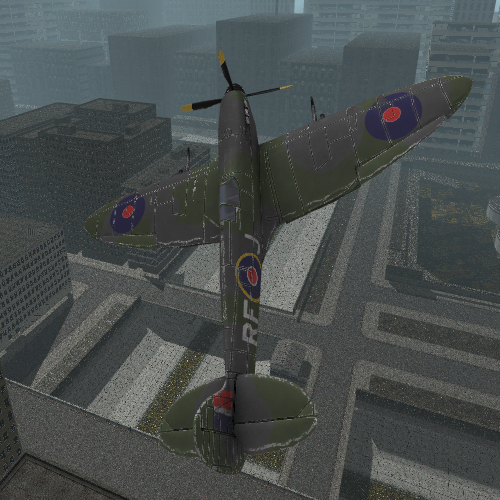
\includegraphics[width=0.45\textwidth]{phongComparison.png}
		& 
		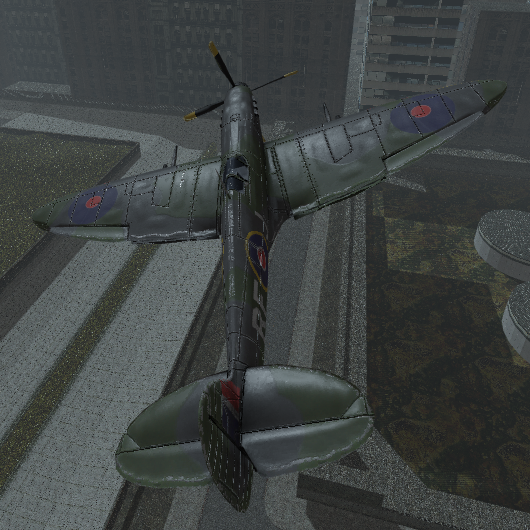
\includegraphics[width=0.45\textwidth]{pbrComparison.png}
		\\
		\caption{Model oświetlony z wykorzystaniem modelu Blinna-Phonga.}
		\label{phongCom}
		&   \caption{Model oświetlony z wykorzystaniem podejścia PBR.}
		\label{pbrCom}
	\end{tabular}
\end{figure}

\subsection{Rysowanie cieni}

Cienie zostały zaimplementowane z wykorzystaniem metody mapowania cieni (ang. shadow mapping) po raz pierwszy zaproponowanej w \cite{shadowmapping}. Polega ona na wyrenderowaniu otoczenia, które chcemy zacieniować z punktu widzenia światła, by potem z wykorzystaniem byfora głębokości, zdecydować czy analizowany fragment znajduje się w cieniu czy nie. Przykładowy bufor głębokości dla światła kierunkowego słońca został przedstawiony na rysunku (\ref{shadowMap}), a efekty takiego podejścia na rysunku (\ref{shadows}).
\\

\begin{figure}[h]
	\centering
	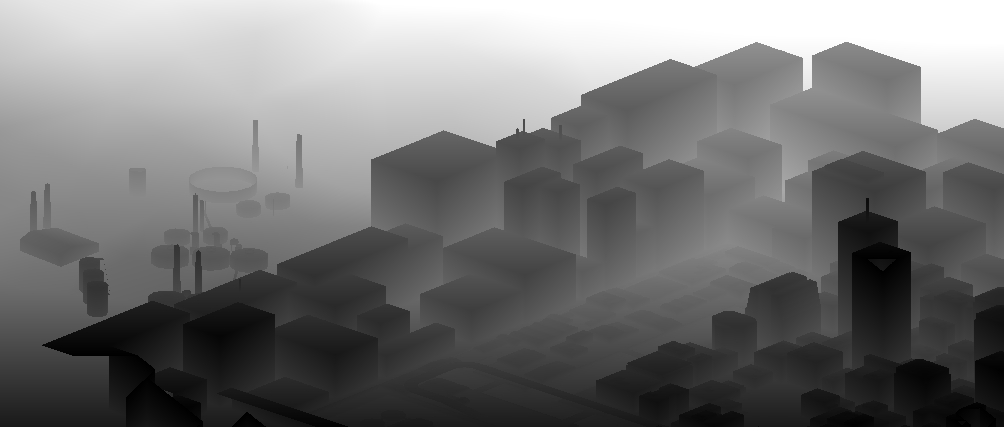
\includegraphics[width=0.9\textwidth]{shadowMap.png}
	\caption{Wycinek mapy głębi wykorzystywanej przy sprawdzaniu czy przetwarzany fragment znajduje się w cieniu.}
	\label{shadowMap}
\end{figure}


\begin{figure}[h]
	\centering
	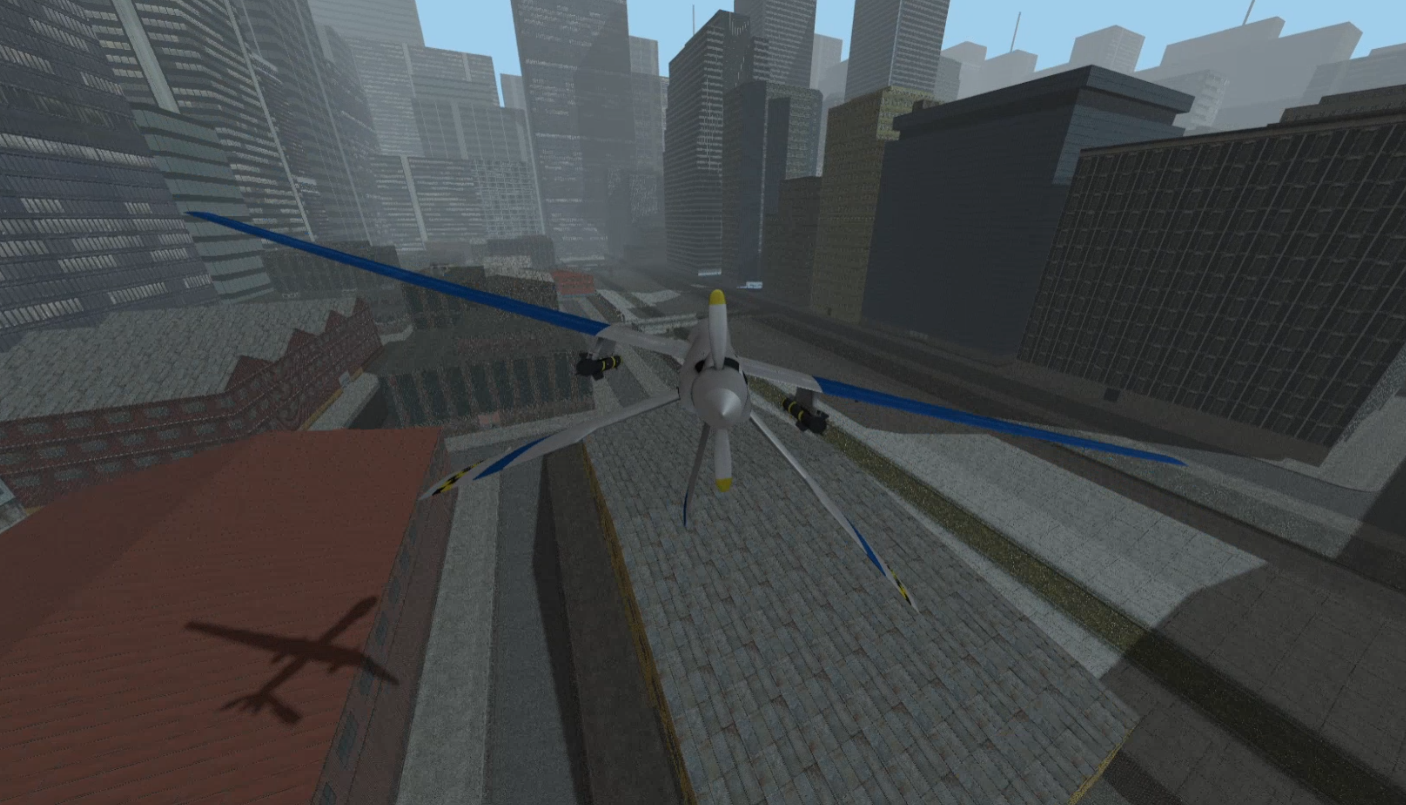
\includegraphics[width=0.9\textwidth]{shadows.png}
	\caption{Cień BSP oraz cienie budynków w oddali narysowane z wykorzystaniem metody shadow mappingu.}
	\label{shadows}
\end{figure}

Pierwszym krokiem w wybranym podejściu jest inicjalizacja tekstury oraz buforu klatki, które będą wykorzystane do rysowania mapy głębi. Rozmiar tekstury jest konfigurowalny, domyślnie ustawiony na 6072x6072 pikseli. Tekstura ma wyłącznie kanał głębokości i bufor klatki ma wyłączone bufory koloru do zapisu oraz odczytu.
\\

Następnie dla każdej klatki, przed wyrenderowaniem domyślnej sceny, wykonywany jest shading pass, a więc renderowanie obiektów na scenie z perspektywy światła na odrębną teksturę. Shader cienia wykonuje wyłącznie transformację do perspektywy ortograficznej, a shader fragmentowy jest wyłączony. Przekształcenie ortograficzne należy dostosować do mapy poprzez zmianę głębokości, która zostanie objęta, ponieważ większe, dalej położone obiekty mogą zostać obcięte z tekstury i przestać rzucać cień. Z powodu ograniczenia na rozmiar tekstury mapa porusza się wraz ze BSP użytkownika. 
\\

Wygenerowana mapa cieni jest następnie przekazywana do głównego shadera. Tam, dla każdego fragmentu, próbkowana jest wartość tekstury dla odpowiednio zmapowanych współrzędnych. W ten sposób determinowane jest czy dany fragment zostanie oświetlony czy nie. 
Aby uniknąć efektu tzw. shadow acne, a więc sytuacji spowodowanej ograniczoną rozdzielczością mapy cieni. Niektóre fragmenty, na które światło pada pod większym kątem, mogą próbkować tą samą wartość teksela. Jednocześnie jedne z nich test głębokości przejdą, a drugie nie. Z tego powodu można otrzymać efekt, który został zilustrowany na rysunku (\ref{shadow_mapping_acne_diagram}). Aby temu zaradzić, jednym z rozwiązań jest zwiększenie błędu testu dla powierzchni, których wektor normalny jest pod większym kątem w stosunku do źródła światła, co daje rezultat jak na rysunku (\ref{shadow_mapping_acne_bias})
\\

\begin{figure}[h]
	\centering
	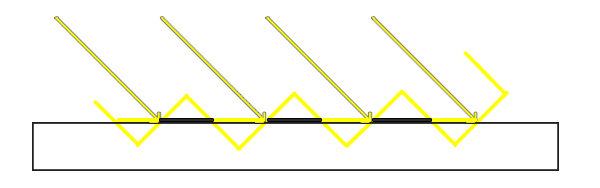
\includegraphics[width=0.6\textwidth]{shadow_mapping_acne_diagram.png}
	\caption{Schemat przedstawiający problem tzw. shadow acne, podczas implementacji metody shadow mappingu \cite{learnopengl}.}
	\label{shadow_mapping_acne_diagram}
\end{figure}

\begin{figure}[h]
\centering
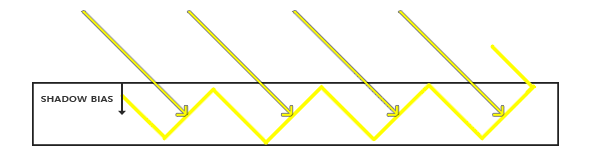
\includegraphics[width=0.6\textwidth]{shadow_mapping_acne_bias.png}
\caption{Schemat rozwiązania problemu shadow acne z wykorzystaniem większego błędu testu głębokości dla powierzchni o większym nachyleniu w stosunku do światła \cite{learnopengl}.}
\label{shadow_mapping_acne_bias}
\end{figure}

Ostatecznie, w celu uniknięcia ostrych krawędzi cieni, zdecydowano się na zastosowanie metody PCF (ang. percentage-closer filtering), która próbkuje dodatkowo 8 tekseli mapy cieni wokół analizowanego fragmentu. Wartości te następnie są uśredniane, uzyskując tym samym częściowe zacienienie.

\subsection{Rysowanie obwódki modelu za ścianą}

Jednym z pierwszych problemów wizualizacji był brak widoczności modelu BSP użytkownika gdy między nim, a kamerą znajdowała się przeszkoda. Zdecydowano się na rozwiązanie tego problemu za pomocą zielonej obwódki wokół modelu jak widać na rysunku (\ref{outline}). Efekt ten został osiągnięty z wykorzystaniem dodatkowej maski widocznej na rysunku (\ref{outlineDebug}) oraz manipulacji buforu głębokości oraz buforu szablonowego.
\\

Bufor szablonowy (ang. stencil buffer) umożliwia selektywne wyświetlanie wybranych pikseli obrazu. Gdy bufor szablonowy jest włączony, to to czy piksel zostanie narysowany determinuje funkcja testu na odpowiadającej mu wartości bufora. Do funkcji należą porównania z wykorzystaniem relacji równości i nierówności oraz funkcje, które przechodzą zawsze lub nigdy.
Dodatkowo, każdy fragment może wpłynąć na bufor. Programista może wybrać operację, jaka ma zostać wykonana w trzech przypadkach: test szablonu nie przeszedł pomyślnie, test szablonu powiódł się, ale nie test głębokości oraz gdy obydwa testy się powiodły. Do operacji należą wyzerowanie wartości, zanegowanie, zinkrementowanie bądź zdekrementowanie, ustalenie jej na konkretną wartość lub pozostawienie bez zmian. Domyślną operacją dla wszystkich przypadków jest pozostawienie wartości bez zmian. Dodatkowe możliwości daje też maska bitowa, która decyduje o tym, jakie bity pikselu bufora będą sprawdzane i modyfikowane. 
\\

Zatem, aby otrzymać efekt jak na rysunku (\ref{outline}), należy wyrenderować środowisko, narysować obwódkę tylko tam, gdzie BSP użytkownika jest zasłonięty przez obiekty środowiska i ostatecznie narysować sam statek. Samo zastosowanie odwróconego testu głębokości nie jest wystarczające, ponieważ obwódka po wyrenderowaniu będzie miała taki sam poziom głębokości jak statek przez co zostanie nadpisana. Aby temu uniknąć, wykorzystany zostanie bufor szablonowy, który pozwoli na wykluczenie fragmentów należących do obwódki w drugim renderowaniu.
\\

Pierwszym krokiem wybranego podejścia jest aktywacja testu buforu szablonowego w OpenGL oraz utworzenie tekstury maski o rozmiarze ekranu i podpięcie jej pod dedykowany bufor ramki. Następnie inicjalizowane są shadery. Shader maski jest prostym programem, który przekształca model do przestrzeni rzutowej i koloruje wszystkie fragmenty na jednolity kolor. Shader obwódki jest bardziej skomplikowany. Po przekształceniu wierzchołków do przestrzeni rzutowej próbkowane są wartości tekseli maski wokół obecnie przetwarzanego fragmentu. Wartości te porównywane są z wartością maski, w miejscu, na który mapuje się fragment i znajdowana jest największa różnica. Gdy różnica przekracza ustaloną granicę, w przypadku naszej implementacji $0.2$, to fragment staje się częścią obwódki i jest kolorowany na zielono.
\\

Proces renderowania obwódki dla każdej klatki obrazu rozpoczyna się od wyczyszczenia buforu maski i wygenerowania nowej na podstawie wyłącznie modelu obecnie kontrolowanego BSP. Wynikiem tej operacji jest jednokolorowy obraz statku w przestrzeni rzutu na czarnym tle. 
Następnie, obok buforu koloru i głębokości, czyszczony jest bufor szablonowy ramki głównej sceny. 
Najpierw rysowane jest symulowane środowisko z wyzerowaną maską buforu szablonowego. Uniemożliwia to wpłynięcie na jego zawartość. 
Maska jest przywracana do maksymalnej wartości, funkcja buforu jest ustawiana na test przechodzący zawsze, operacja zamiany na ustalenie wartości $1$ gdy obydwa testy przechodzą pomyślnie. Test głębokości został ustawiony na pomyślny, gdy testowana wartość jest większa od obecnej. Z taką konfiguracją rysowany jest BSP użytkownika z wykorzystaniem shadera obramówki. 
Efektem jest zielona obramówka na ekranie tam, gdzie statek jest obecne zakryty, bufor głębokości środowiska zmodyfikowany o głębokość statku za ścianą oraz bufor szablonowy z wartościami $1$ tamże.
Statek jest rysowany ponownie za pomocą domyślnego shadera, z funkcją przechodzącą, wtedy gdy wartość bufora szablonowego jest równa $0$, wyłączoną modyfikacją tego buforu i domyślnym testem głębokości. W rezultacie otrzymany zostanie poprawnie narysowany statek z obwódką za przeszkodami. Ostatecznie bufor szablonowy jest wyłączany do momentu rozpoczęcia przetwarzania następnej klatki, a reszta sceny jest renderowana bez zmian.

\begin{figure}[h]
	\centering
	\setkeys{Gin}{width=\textwidth}
	x\begin{tabular}{p{0.45\textwidth}p{0.45\textwidth}}
		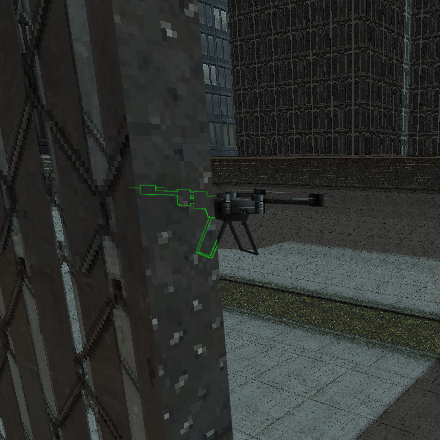
\includegraphics[width=0.45\textwidth]{outline.png}
		& 
		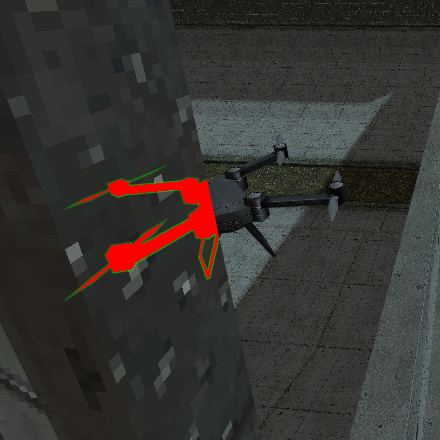
\includegraphics[width=0.45\textwidth]{outlineDebug.png}
		\\
		\caption{Zielona obwódka jest widoczna, gdy między BSP użytkownika a kamerą znajduje się przeszkoda.}
		\label{outline}
		&   
		\caption{Zielona obwódka wraz z maską wykorzystywaną do jej obliczenia.}
		\label{outlineDebug}
	\end{tabular}
\end{figure}

\subsection{Ślad po wystrzelonym pocisku}

Przy implementacji pocisków zauważono, że małe pociski przy odpowiednio wysokiej prędkości są praktycznie niezauważalne. Dotyczy to na przykład nabojów wystrzelonych z broni palnej. Sam model pojawia się na ekranie wyłącznie przez kilka klatek. Aby temu zaradzić, zdecydowano się na dodanie śladu podążającego za pociskami. Jest to oddzielny shader operujący bez bufora wierzchołkowego. Shader jest uruchamiany dla każdego pocisku i wykorzystuje $n$ ostatnio zapisanych pozycji. Na ich podstawie shader geometrii tworzy line strip rozpoczynający się od obecnej pozycji pocisku i kończący na ostatnim zapisanym punkcie zwiększając w każdym węźle przezroczystość linii. Dzięki zastosowaniu śladu pocisku użytkownik jest w stanie lepiej zorientować się, w jakim kierunku pocisk poleciał, a nawet zauważyć potencjalne rykoszety związane z mechanizmem wykrywania kolizji jak widać na rysunku (\ref{rykoszet}).

\begin{figure}[h]
	\centering
	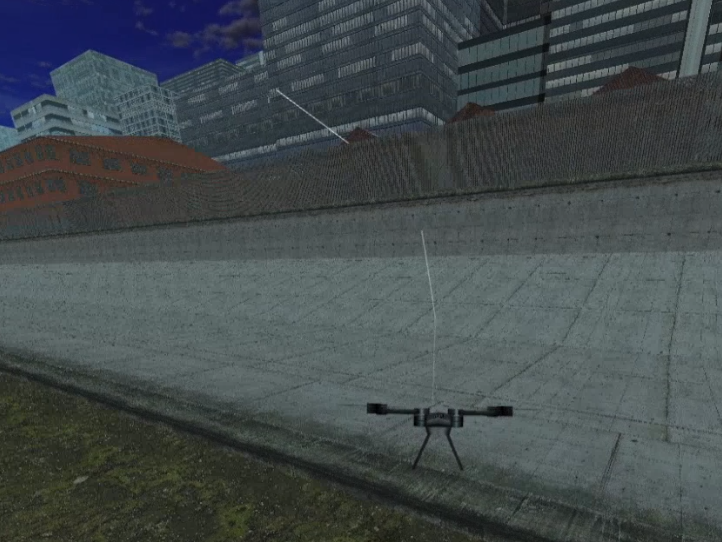
\includegraphics[width=0.5\textwidth]{rykoszet.png}
	\caption{Ślad pocisku pokazujący podwójny rykoszet pocisku.}
	\label{rykoszet}
\end{figure}

\subsection{Rysowanie liny}

Ładunek zrzucany przez BSP początkowo jest umocowany na linie. Serwer jest odpowiedzialny za jej fizykę, przekazując wizualizacji informacje o tym, gdzie w danej chwili znajdują się końce liny oraz jej długość. Z taką ilością informacji zdecydowano się na zamodelowanie obiektu trójwymiarowego za pomocą krzywej łańcuchowej. Efekty podejścia można zobaczyć na rysunku (\ref{gui_game4})
\\

\begin{figure}[!h]
	\centering
	\includegraphics[width=1\textwidth]{game\_view\_rope.png}
	\caption{Wizualizacja w widoku obserwatora i pozycyjnym trybie lotu z opuszczonym ładunkiem na linie.}
	\label{gui_game4}
\end{figure}

Krzywa łańcuchowa, wyrażona za pomocą wzoru przeskalowanego cosinusa hiperbolicznego, określa kształt jaki przyjmuje doskonale nierozciągliwa lina o jednakowo rozłożonej niezerowej masie, zawieszona między dwoma punktami w jednorodnym polu grawitacyjnym. Wzór ten przyjmuje postać:

\[
	y = a \cosh \left( \frac{x}{a} \right).
\]

Wyznaczenie współczynnika krzywej łańcuchowej $a_c$ między punktami $A = (x_1,y_1)$, $B = (x_2,y_2)$ i danego $l < \lVert B - A \rVert$, to rozwiązanie równania:
\[
	\frac{1}{h} \sqrt{l^2-v^2} = \frac{2a_c}{h} \sinh\left( \frac{h}{2a_c} \right),
\]
gdzie:
$$
h = x_2 - x_1,
$$
$$
v = y_2 - y_1.
$$

Zauważmy, że możemy przyporządkować rozważane punkty do $A$ i $B$ w taki sposób, by $x_1$ było zawsze mniejsze od $x_2$, uzyskując tym samym $h > 0$.
\\

Powyższe równanie nie posiada rozwiązania analitycznego, więc musi ono być rozwiązane metodą numeryczną. Jest to możliwe, ponieważ idąc przykładem \cite{Routh_2013}, możemy zauważyć, że z racji, że $sinh(x)/x$ jest ściśle rosnące dla $x>0$, to istnieje co najwyżej jedno rozwiązanie dla $a>0$. Nie interesuje nas rozwiązanie ujemne $a < 0$, ponieważ oznacza ono odwróconą krzywą łańcuchową. 
\\

Aby zapewnić stabilne wyznaczenie współczynnika możemy zastosować rozwiązanie zaproponowane w \cite{1002996}. Polega ono na przekształceniu równania do następującej postaci:

\[
	\left( \frac{\sqrt{l^2 - v^2}}{h} \right)^{-1/2} = \left( 2b\sinh\frac{1}{2b} - 1 \right)^{-1/2},
\]
gdzie:
$$
b = \frac{a}{h}.
$$

Wykreślenie prawej strony powyższego równania w zależności od $b$ na rysunku (\ref{solvingCatenary}) pozwala zauważyć, że funkcja jest w przybliżeniu liniowa na dużym zakresie argumentów.

\begin{figure}[h]
	\centering
	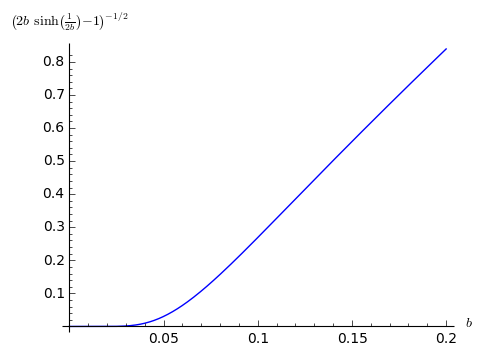
\includegraphics[width=0.5\textwidth]{solvingCatenary.png}
	\caption{Wykreślone równanie. Pozwala zauważyć, że funkcja jest w przybliżeniu liniowa na dużym zakresie argumentów (\cite{1002996}).}
	\label{solvingCatenary}
\end{figure}

Przenosząc lewą stronę na prawo jesteśmy w stanie wykorzystać dowolny algorytm znajdowania miejsc zerowych. 


\[
	\left( 2b\sinh\frac{1}{2b} - 1 \right)^{-1/2} - \left( \frac{\sqrt{l^2 - v^2}}{h} \right)^{-1/2} = 0.
\]

Wybraną metodą została metoda Newtona-Raphsona. Jest to algorytm iteracyjny pozwalający na znalezienie miejsca zerowego funkcji, która na danym przedziale ma tylko jeden pierwiastek, ma różne znaki na końcach przedziału oraz pierwsza i druga pochodna mają stały znak w tym przedziale. Algorytm rozpoczyna się od wybrania wartości początkowej $x_1$, która będzie pierwszym przybliżeniem rozwiązania. Aby obliczyć następne przybliżenie, należy wyznaczyć wartość funkcji oraz jej pochodnej dla $x_1$ i zastosować następujący wzór:

\[
	x_{k+1} = x_k - \frac{f(x_k)}{f'(x_k)},
\]
gdzie $k \in \mathbb{N}$ jest krokiem iteracji .
\\

Wynik wzoru jest brany jako argument następnej iteracji. Proces jest kontynuowany do momentu osiągnięcia warunków końcowych. W naszej implementacji jest to niewielka odległość między kolejnymi przybliżeniami $ | x_{k+1} - x_k | < \varepsilon$, $\varepsilon = 0,001$ oraz maksymalna liczba iteracji $n=1000$.
\\

Proces wyznaczania współczynnika krzywej łańcuchowej rozpoczyna się od zbadania odległości między punktami przytwierdzenia liny. Jeżeli przekracza ona długość liny, to współczynnik jest ustawiany na współczynnik kierunkowy prostej między tymi punktami. Symuluje to napięcie liny w przypadku gdy jest ona rozciągana. Wtedy podejście różni się wyłącznie funkcją wyznaczania wysokości punktów, zatem dla ustalenia uwagi następne akapity dotyczyć będą ciekawszego przypadku gdy odległość jest mniejsza niż długość liny. W tym przypadku zastosowana jest metoda Newtona-Raphsona. Z racji, że punkty są trójwymiarze, wymagana jest odpowiednia interpretacja $v$ i $h$. Załóżmy, że naszymi punktami są $A = (x_A, y_A, z_A)$ oraz $B= (x_B, y_B, z_B)$. Wtedy $v = z_B - z_A$ oraz $ h = \sqrt{(x_B - x_A)^2 + (y_B - y_A)^2}$. Zatem możemy uruchomić algorytm dla następujących wartości:

$$
	f(b) = \left( 2b\sinh\frac{1}{2b} - 1 \right)^{-1/2} - \left( \frac{\sqrt{l^2 - v^2}}{h} \right)^{-1/2},
$$

$$
	f'(b) = \left( \frac{1}{2b} \cosh \frac{1}{2b} - \sinh \frac{1}{2b} \right) \left( 2b \sinh \frac{1}{2b} - 1 \right) ^ {-3/2},
$$

$$
b_1 = 0.05. 
$$

Współczynnik krzywej łańcuchowej można wyznaczyć za pomocą wzoru $a = \frac{b}{h}$.
\\

Do poprawnego narysowania liny brakuje jeszcze wartości przesunięcia, aby wiedzieć jaki fragment krzywej łańcuchowej wykorzystać. W tym celu ponownie zostanie wykorzystana metoda Newtona-Raphsona dla następujących wartości:


$$
f(x) =  a \left( \cosh \frac{p.x + x}{a} - \cosh \frac{x}{a} \right) + p.y,
$$

$$
f'(x) = \sinh \frac{p.x + x}{a} - \sinh \frac{x}{a}
$$

$$
x_1 = p.x / 2,
$$
gdzie
$$
p = (h, v).
$$

Ostatecznie $x_{offset} = x_0$ i $y_{offset} = -a\cosh \frac{x_0}{a}$, dla znalezionego pierwiastka $x_0$.
\\

Mając wszystkie niezbędne dane do określenia punktów na krzywej łańcuchowej, opisane zostanie jak punkty te zostaną przedstawione w trójwymiarze. Model liny będzie bryłą złożoną z $N$ segmentów, z których każdy będzie przybliżeniem cylindra ściętego z obu stron. Podstawy są przybliżone za pomocą wielokąta foremnego, a powierzchnia każdej z nich jest prostopadła do wektora stycznego z krzywą łańcuchową w danym punkcie. Zostało to zaprezentowane na schemacie (\ref{rope_model}).
\\

\begin{figure}[h]
	\centering
	\includegraphics[width=0.5\textwidth]{rope\_model.png}
	\caption{Model liny złożony z segmentów w kształcie przybliżonych cylindrów ściętych z obu stron.}
	\label{rope_model}
\end{figure}

Z racji, że kształt liny będzie się dynamicznie zmieniał w czasie w celu narysowania powyższego modelu, oprócz shadera wierzchołkowego i fragmentowego, zdecydowano się na wykorzystanie shadera geometrii. Na wejściu otrzymuje on dwie liczby z przedziału $[0, 1]$. Reprezentują one dwa punkty tworzące jeden z segmentów modelu w postaci odległości poziomej do jednego z końców podzielonej przez całkowitą odległość poziomą między końcami liny. Mając te dane oraz współczynnik krzywej łańcuchowej oraz przesunięcia argumentów i wartości, shader może wyznaczyć położenia punktów w trójwymiarze. 
\\

Następnym krokiem obliczania modelu liny jest wyznaczenie wierzchołków bryły. Do znalezienia punktów podstawy zdecydowano się na wyznaczenie wektora normalnego oraz obrócenie go $k$ razy wokół osi wektora stycznego za pomocą formuły obrotu Rodrigues'a, gdzie $k$ to jest liczba kątów wielokąta foremnego. 

\begin{equation*}
	\frac{d}{dx} \left( a \cosh \frac{x}{a} \right) = \sinh \frac{x}{a}
\end{equation*}
\begin{equation*}
	\vec{t} =
	\begin{pmatrix}
		1 \cdot \frac{|\vec{l_x}|}{\vec{|l_{xy}}|}, &
		1 \cdot \frac{|\vec{l_y}|}{\vec{|l_{xy}}|}, &
		-\sinh\frac{x}{a}
	\end{pmatrix}^T
\end{equation*}
\begin{equation*}
	\vec{n_0} =
	\begin{pmatrix}
		\sinh \frac{x}{a} \cdot \frac{|\vec{l_x}|}{\vec{|l_{xy}}|}, &
		\sinh \frac{x}{a} \cdot \frac{|\vec{l_y}|}{\vec{|l_{xy}}|}, &
		1
	\end{pmatrix}^T
\end{equation*}

\begin{equation*}
	W_R = 
	\begin{pmatrix}
		0 & -\vec{t_z} & \vec{t_y} \\
		\vec{t_z} & 0 & -\vec{t_x} \\
		-\vec{t_y} & \vec{t_x} & 0 \\
	\end{pmatrix}
\end{equation*}
\begin{equation*}
	M_R = I + sin \left(\frac{2\pi}{k} \right) \cdot W_R + 2\sin^2 \left(\frac{\pi}{k} \right) \cdot W_R^2
\end{equation*}
\begin{equation*}
	\forall_{i=1,2,\cdots, k} \hspace{1em} \vec{n_i} = \vec{n_0} \cdot M_R^i
\end{equation*}

Ostatecznie każde uruchomienie shadera geometrii tworzy siatkę trójkątów utworzonych z $2(k+1)$ punktów wokół punktów $p_n$ i $p_{n+1}$ formatu $p_n^{(i)} = p_n + n_i$, gdzie $p_n$ to punkt rozpoczynający n-ty fragment modelu. Są one następnie przekształcane do przetrzeni rzutowej i standardowo cieniowane w etapie shadera fragmentowego.

\subsection{Animacja modelu}

Dzięki temu, że wizualizacja opiera się na modelach w formacie glTF, możliwe jest zdefiniowanie oraz wykorzystanie animacji. Animacje są obsługiwane za pomocą prostego interfejsu. Udostępnia on wszystkie animacje dostępne w modelu pod nazwą podmodelu, który jest animowany, czas trwania animacji oraz liczbę w przedziale $[0,1]$, która oznacza, którą klatkę w danej chwili wybrać. W ten sposób można identyfikować kategorie animacji oraz ustalać ich przebieg. Obecnie obsługiwane są:
\begin{enumerate}
	\item modele śmigieł, które przypisane są kolejnym śmigłom BSP w kolejności alfabetycznej. Obracają się one z prędkością liczby obrotów na minutę oryginalnych śmigieł,
	\item modele steru kierunku, wysokości oraz lotki, które są przypisane do odpowiadających osi kontrolera,
	\item oraz modele ładunków, które są przypisane do ładunku znajdującego się w konfiguracji statku. Gdy zostanie on wystrzelony bądź opuszczony, skala modelu zostaje ustawiona na $0$, w efekcie sprawiając, że model staje się niewidzialny.
\end{enumerate}

\addtocontents{toc}{\protect\newpage}
\section{Graficzny interfejs użytkownika}

Graficzny interfejs użytkownika został zaprojektowany z myślą o zaprezentowaniu jak największej ilości informacji, nie tracąc na przejrzystości przekazu.
\\

Został on zaimplementowany z wykorzystaniem czterech shaderów. Wszystkie z nich rysują płaski obraz bez testu głębokości. Shader sprite'ów umożliwia rysowanie tekstury na prostokącie (ang. quad) poddanej pewnym transformacjom oraz o danym poziomie transparentności. Z jego pomocą rysowane są bardziej skomplikowane elementy niewymagające złożonych transformacji. Shader pozwala na rysowanie dowolnej płaskiej geometrii w jednolitym kolorze. Jest on wykorzystywany do prostokątów, trójkątów oraz kół. Shader wycinka koła jest specjalizacją shadera wektorowego, która pozwala dodatkowo ustawić kąt, w którym wycinek się rozpoczyna oraz kończy. Przyjmuje on na wejściu koło odrzucając fragmenty niespełniające predykatu. Shader tekstu umożliwia wyświetlenie dowolnego ciągu znaków za pomocą wybranego fontu TrueType. Każdy glif jest wyświetlany na prostokącie dopasowanym do jego rozmiarów. Z aplikacją dostępny jest font FreeSans.

\subsection{Sztuczny horyzont}

Najważniejszym komponentem interfejsu jest sztuczny horyzont widoczny na rysunkach (\ref{horizon1}) i (\ref{horizon2}). Jego wygląd i działanie odpowiada typowemu wyposażeniu statków powietrznych w standardzie NATO, gdzie symbol statku jest nieruchomy, a wyświetlany horyzont utrzymuje się zgodnie z horyzontem naturalnym widocznym z perspektywy pilota. Z widżetu możemy się dowiedzieć o obecnym przechyleniu, pochyleniu oraz odchyleniu statku w stopniach, o jego prędkości poziomej na panelu po lewej stronie i wysokości po prawej jak i o jego położeniu oraz prędkości wznoszenia (ang. climb rate). Ponadto w lewym górnym rogu widnieje informacja o obecnym trybie kontroli lotu. Tryb ten warunkuje jakie wartości z wyżej wymienionych są przez niego narzucane, a więc i wyświetlane w postaci odpowiedniej nakładki jak na rysunku (\ref{horizon2}).




\begin{figure}[h]
	\centering
	\setkeys{Gin}{width=\textwidth}
	\begin{tabular}{p{0.45\textwidth}p{0.45\textwidth}}
		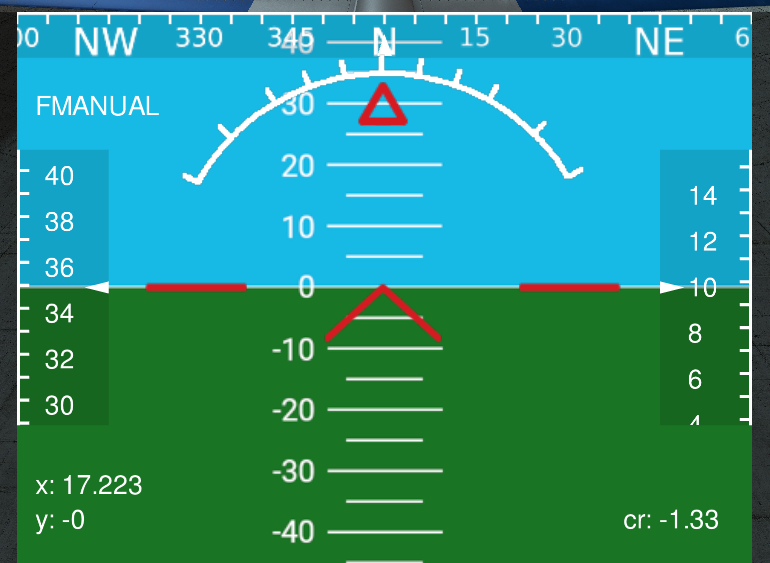
\includegraphics[width=0.45\textwidth]{horizon1.png}
		& 
		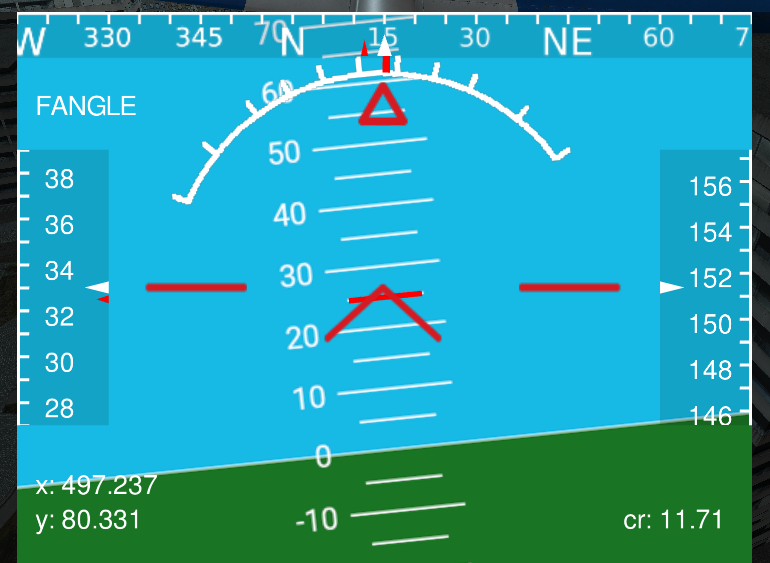
\includegraphics[width=0.45\textwidth]{horizon2.png}
		\\
		\caption{Sztuczny horyzont w domyślnej pozycji podczas startu BSP.}
		\label{horizon1}
		&   
		\caption{Sztuczny horyzont w czasie lotu BSP z zaznaczonymi wartościami zadanymi przez tryb kontroli lotu.}
		\label{horizon2}
	\end{tabular}
\end{figure}

\subsection{Wyznaczenie parametrów panelu śmigieł}

Panel śmigieł jest komponentem pomagającym na zorientowanie się w prędkości obrotowej każdego z rotorów BSP. Pokazana jest dokładna liczba obrotów na minutę wraz z wizualizacją przedstawiającą prędkość względem prędkości maksymalnej. Ponadto uwzględnione jest czy śmigło obraca się zgodnie, czy przeciwnie do wskazówek zegara. Wygląd panelu jest pokazany na rysunku (\ref{smigla}). Położenie śmigieł na panelu jest generowane proceduralnie na podstawie konfiguracji BSP podczas inicjalizacji aplikacji. Algorytm bierze pod uwagę konfigurację panelu w postaci marginesu oraz paddingu poszczególnych śmigieł oraz wysokość i minimalną szerokość okna tekstu. Zwraca uwagę również na odległości względne śmigieł w konfiguracji statku. Na rysunku (\ref{smiglaDebug}) został zaprezentowany podgląd deweloperski panelu, który koloruje poszczególne jego części, a na rysunku (\ref{smiglaDebugRandom}) pokazane są możliwości algorytmu dla losowego rozmieszczenia śmigieł na BSP.
\\

Początkowo próbowano znaleźć parametry panelu za pomocą równań matematycznych. Z powodu skomplikowanych zależności zdecydowano się na podejście iteracyjne, które byłoby uruchamiane raz podczas inicjalizacji aplikacji. Zaprojektowany algorytm wykorzystuje podejście "dziel i zwyciężaj" szukając rozwiązanie w pikselach na przedziale $[1,\text{canvasSize}/2]$. Program bierze środkowy element obecnie analizowanego przedziału i sprawdza, czy wybrany promień się mieści w ustalonych ograniczeniach. Jeżeli się udaje, to próbuje promień większy w podprzedziale z prawej strony elementu, w przeciwnym wypadku rozmiar mniejszy w podprzedziale z lewej strony.


\begin{figure}[h]
	\centering
	\setkeys{Gin}{width=\textwidth}
	\begin{tabular}{p{0.45\textwidth}p{0.45\textwidth}}
		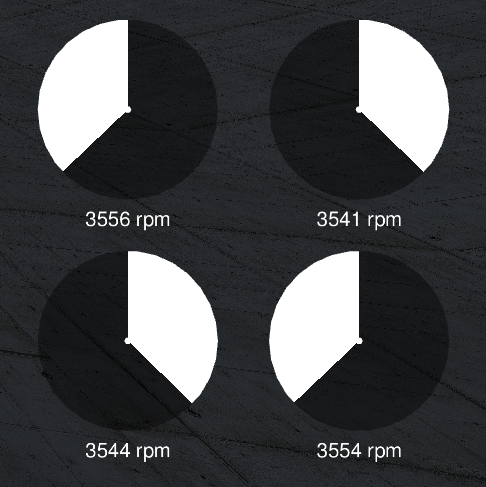
\includegraphics[width=0.45\textwidth]{smigla.png}
		& 
		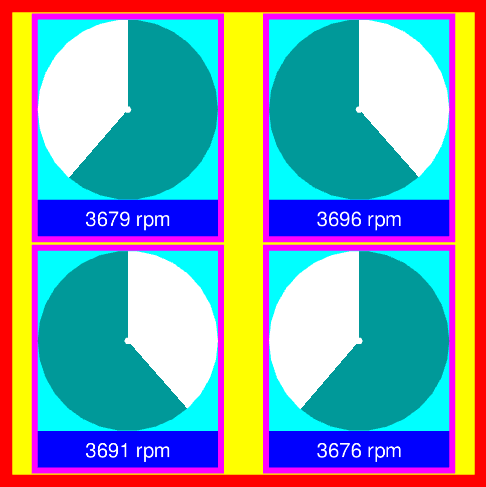
\includegraphics[width=0.45\textwidth]{smiglaDebug.png}
		\\
		\caption{Panel śmigieł jak widoczny w wizualizacji.}
		\label{smigla}
		&   \caption{Panel śmigieł w trybie deweloperskim pokazujący margines, padding oraz miejsce przeznaczone na poszczególne śmigła oraz tekst.}
		\label{smiglaDebug}
	\end{tabular}
\end{figure}

\begin{figure}[h]
	\centering
	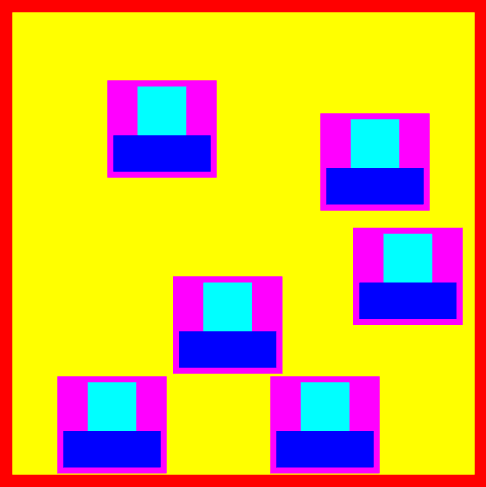
\includegraphics[width=0.5\textwidth]{smiglaDebugRandom.png}
	\caption{Panel śmigieł w trybie deweloperskim. Pokazanie możliwości algorytmu generowania dla losowego rozmieszczenia śmigieł. Są zachowane odległości i uwzględniona  jest minimalna szerokość panelu tekstu.}
	\label{smiglaDebugRandom}
\end{figure}

\subsection{Panel komunikatów}

W aplikacji znajdują się dwa panele komunikatów. Panel komunikatów krytycznych wyświetlany jest na środku ekranu dużą czcionką, pokazując wyłącznie najnowszy komunikat z danej kategorii. Obsługuje on ostrzeżenia, na które pilot musi niezwłocznie zareagować. Jest wykorzystywany przez serwer do informowania użytkownika o rozpoczęciu lotu, kolizjach i przekroczeniu bezpiecznej wartości przeciążenia. Ostrzega również o zbliżaniu się do granicy terenu symulacji oraz informuje o usunięciu statku, gdy ten poza teren wyleci. Jest on zaprezentowany na rysunku (\ref{fig:critical}).
\\

\begin{figure}
	\centering
	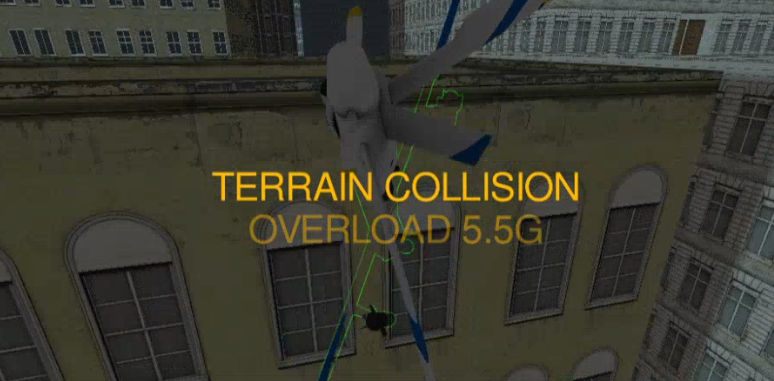
\includegraphics[width=0.7\linewidth]{critical.png}
	\caption{Panel komunikatów krytycznych informujący o zderzeniu oraz przeciążeniu 5.5G przekraczającego bezpieczną wartość przyspieszenia.}
	\label{fig:critical}
\end{figure}

Panel komunikatów niekrytycznych wyświetla się z boku po lewej stronie ekranu. Oprócz wiadomości pokazywany jest również czas jej otrzymania od momentu uruchomienia aplikacji. Jest to medium komunikacji między wizualizacją, a użytkownikiem. Informować on może m.in. o włączeniu muzyki, odpowiedziach serwera na akcje użytkownika jak na przykład zbyt wiele jednoczesnych próśb o restart lotu BSP i liście dostępnych amunicji do wybrania. Przykłady powyższych wiadomości zostały pokazane na rysunkach (\ref{logExample}) i (\ref{logAmmo}).

\begin{figure}
	\centering
	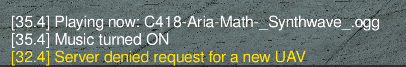
\includegraphics[width=0.7\linewidth]{logExample.png}
	\caption{Panel komunikatów wyświetlający dostępną amunicję wraz z obecnie wybraną.}
	\label{logExample}
\end{figure}

\begin{figure}
	\centering
	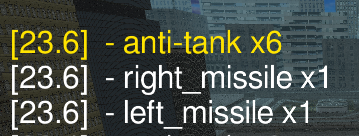
\includegraphics[width=0.4\linewidth]{logAmmo.png}
	\caption{Panel komunikatów wyświetlający dostępną amunicję wraz z obecnie wybraną.}
	\label{logAmmo}
\end{figure}


\subsection{Radar}

Radar umożliwia użytkownikowi zorientować się w obecności innych BSP w najbliższej okolicy. Symulowane jest działanie radaru aktywnego uwzględniające aktualną orientację statku oraz ramienia radaru. Inne BSP na radarze wyświetlane są jako kropki po pewnym czasie zanikające. Został on zilustrowany na rysunku (\ref{radar}).


\begin{figure}[h]
	\centering
	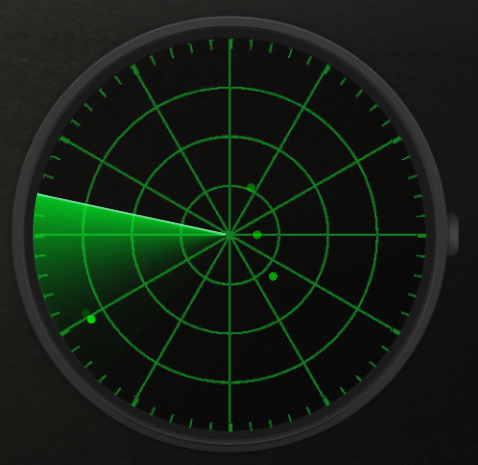
\includegraphics[width=0.5\textwidth]{radar.png}
	\caption{Radar z paroma wykrytymi BSP.}
	\label{radar}
\end{figure}

\subsection{Ekran ładowania oraz ekran generatora przypisań kontrolera}
	
Ekran ładowania wyświetlany jest w momencie uruchomienia aplikacji i ma za zadanie poinformować użytkownika o postępie ładowania zawartości. Spełnia on również dodatkową rolę, upewniając użytkownika, że program się nie zawiesił, ponieważ w zależności od wagi wczytywanych tesktur, ładownie może trwać do kilkunastu sekund. Przykład został pokazany na rysunku (\ref{gui_loading}).

\begin{figure}[!h]
	\centering
	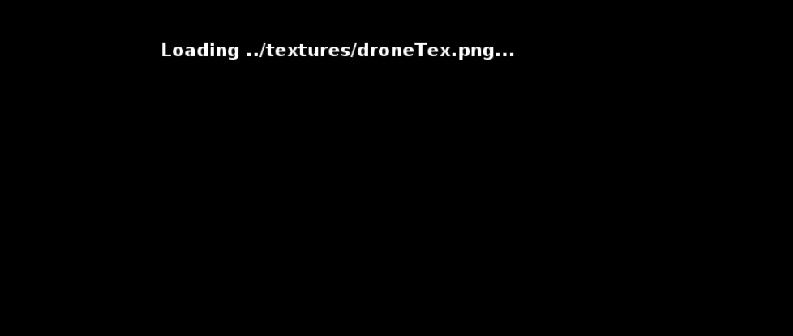
\includegraphics[width=1\textwidth]{loading_screen.png}
	\caption{Ekran ładowania.}
	\label{gui_loading}
\end{figure}

Ekran generatora przypisań kontrolera pojawia się gdy użytkownik ustawił odpowiednią flagę w konfiguracji aplikacji i odpowiada za przeprowadzenie użytkownika przez proces konfiguracji kontrolera. Jest to rozwiązanie związane z nieograniczaniem się do powszechnie używanych modeli kontrolerów. Dzięki temu możliwe jest wykorzystanie profesjonalnych kontrolerów prawdziwych BSP. Przykładowy ekran został zaprezentowany na rysunku (\ref{gui_bindings1}).

\begin{figure}[!h]
	\centering
	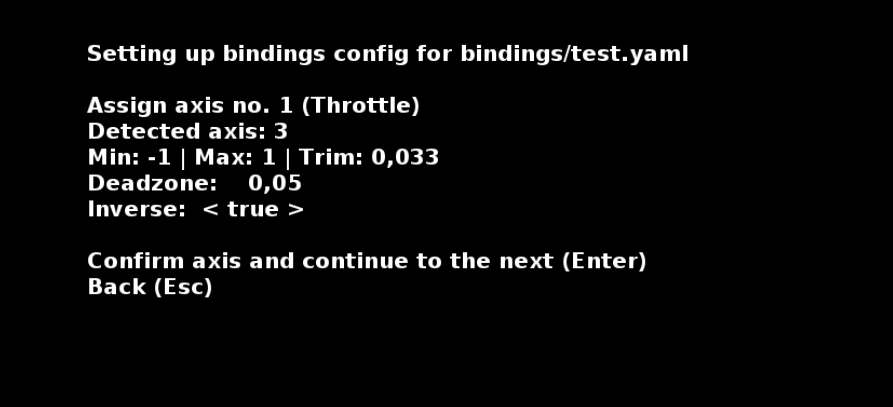
\includegraphics[width=1\textwidth]{bindings1.png}
	\caption{Ekran generatora przypisań kontrolera podczas przypisania osi sterowania.}
	\label{gui_bindings1}
\end{figure}

\subsection{Reszta widżetów}

Użytkownik ma możliwość otworzenia mapy, która ilustruje teren wokół BSP. Można z niej odczytać położenie oraz orientację horyzontalną kontrolowanego statku patrząc na białą ikonę, jak i te zadane przez tryb kontroli lotu patrząc na czerwoną. Ponadto widoczne są kierunek oraz względna wartość prędkości w postaci żółtego wektora. Przykład wyświetlonej mapy zaprezentowano na rysunku (\ref{map})
\\

\begin{figure}[h]
	\centering
	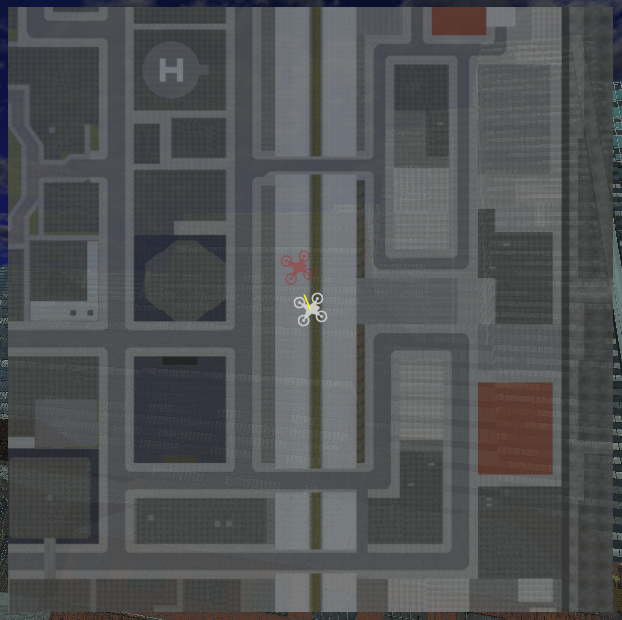
\includegraphics[width=0.7\textwidth]{map.png}
	\caption{Mapa pokazuje okoliczny teren, położenie oraz orientację horyzontalną kontrolowanego statku (biała ikona) jak i te zadane przez tryb kontroli lotu (czerwona ikona) oraz prędkość BSP (żółty wektor).}
	\label{map}
\end{figure}


Do widżetów należy również opcjonalny panel deweloperski pozwalający na podejrzenie średniego czasu renderowania klatek w klatkach na sekundę i milisekundach na klatkę oraz panel z obecnie wybranym pociskiem i ładunkiem wraz z pozostałą liczebnością i czasem do ich przeładowania w postaci wycinku koła. Zostały one zaprezentowane na rysunkach kolejno (\ref{debugPanel}) i (\ref{ammoPanel}).



\begin{figure}[h]
	\centering
	\setkeys{Gin}{width=\textwidth}
	\begin{tabular}{p{0.45\textwidth}p{0.45\textwidth}}
		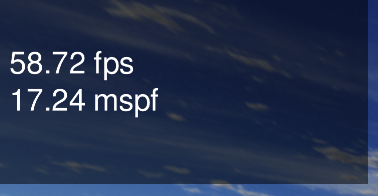
\includegraphics[width=0.45\textwidth]{debugPanel.png}
		& 
		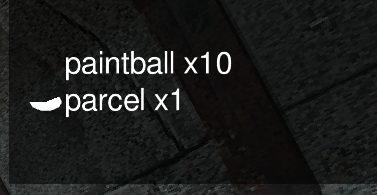
\includegraphics[width=0.45\textwidth]{ammoPanel.png}
		\\
		\caption{Panel deweloperski z liczbą klatek na sekundę i milisekund na klatkę.}
		\label{debugPanel}
		&   \caption{Panel obecnie wybranego pocisku i ładunku wraz z pozostałą liczebnością i czasem do ich przeładowania w postaci wycinka koła.}
		\label{ammoPanel}
	\end{tabular}
\end{figure}

\section{Udźwiękowienie}

Udźwiękowienie symulatora zostało zrealizowane za pomocą implementacji standardu OpenAL. Dzieli się ono na muzykę oraz dźwięk śmigieł. Muzyka, która jest odtwarzana w tle, jest pobierana z katalogu wyznaczonego przez użytkownika losowo wybierając utwory w momencie, gdy poprzedni się zakończy. Użytkownik również odpowiada za uzupełnienie folderu plikami o formacie OGG, które będą odtwarzane. Dźwięk śmigieł natomiast jest częścią symulacji i wykorzystuje bardziej zaawansowane funkcjonalności OpenAL. 
\\

Każdy dźwięk w OpenAL może być reprezentowany przez jego położenie, prędkość, głośność oraz wysokość. W ten sposób każde śmigło może wygenerować swój własny dźwięk. Ma on swoje położenie wyznaczane z wykorzystaniem parametru przesunięcia śmigła względem środka BSP i pozycji samego BSP w świecie oraz prędkość, która dla uproszczenia jest prędkością statku. Uznano, że głośność oraz wysokość dźwięku śmigła jest proporcjonalna do liczby obrotów na sekundę, gdzie dźwięk jest tym głośniejszy i wyższy, im szybciej śmigło się obraca. Z racji, że głośności różnych źródeł dźwięku się sumują, zdecydowano się, w celu zwiększenia komfortu pracy, na znormalizowanie głośności poprzez podzielenie jej przez liczbę rotorów BSP. 
\\

W OpenAL istnieje również koncept słuchacza, który tak samo jak źródło ma swoją pozycję oraz prędkość. Jest ona zawsze ustawiana na obecne położenie oraz prędkość kamery. Dzięki temu głośność dźwięku słyszanego przez użytkownika jest odwrotnie proporcjonalna do odległości kamery od źródła oraz zaobserwować można efekt stereo, co jest najbardziej odczuwalne w kamerze pierwszosobowej, jak i efekt Dopplera.
\\